\section{Zielsetzung}

In diesem Versuch soll durch Beobachtung des Phasenübergangs die 
Verdampfungswärme von Wasser bestimmt werden. Dafür wird die Dampfdruckkurve zu Hilfe genommen.
Außerdem soll dabei die Temperaturabhängigkeit nicht vernachlässigt werden.
Dazu wird der Vorgang der Phasenumwandlung von fest zu flüssig untersucht.
\section{Theoretische Grundlagen}

\subsection{Phasendiagramm}

Die \glqq Phase\grqq{} eines Stoffes beschreibt in diesem Fall den Aggregatzustand.Unterscheiden wird dieser zwischen fest, 
flüssig und gasförmig.
Zur Veranschaulichung wird hier ein Phasendiagramm von Wasser genutzt in dem der Druck gegen die Temperatur aufgetragen ist und die 3 
\glqq Phasen\grqq{} durch 3 Kurven voneinander abgegrenzt sind.\\
\begin{figure}[H]
    \centering
    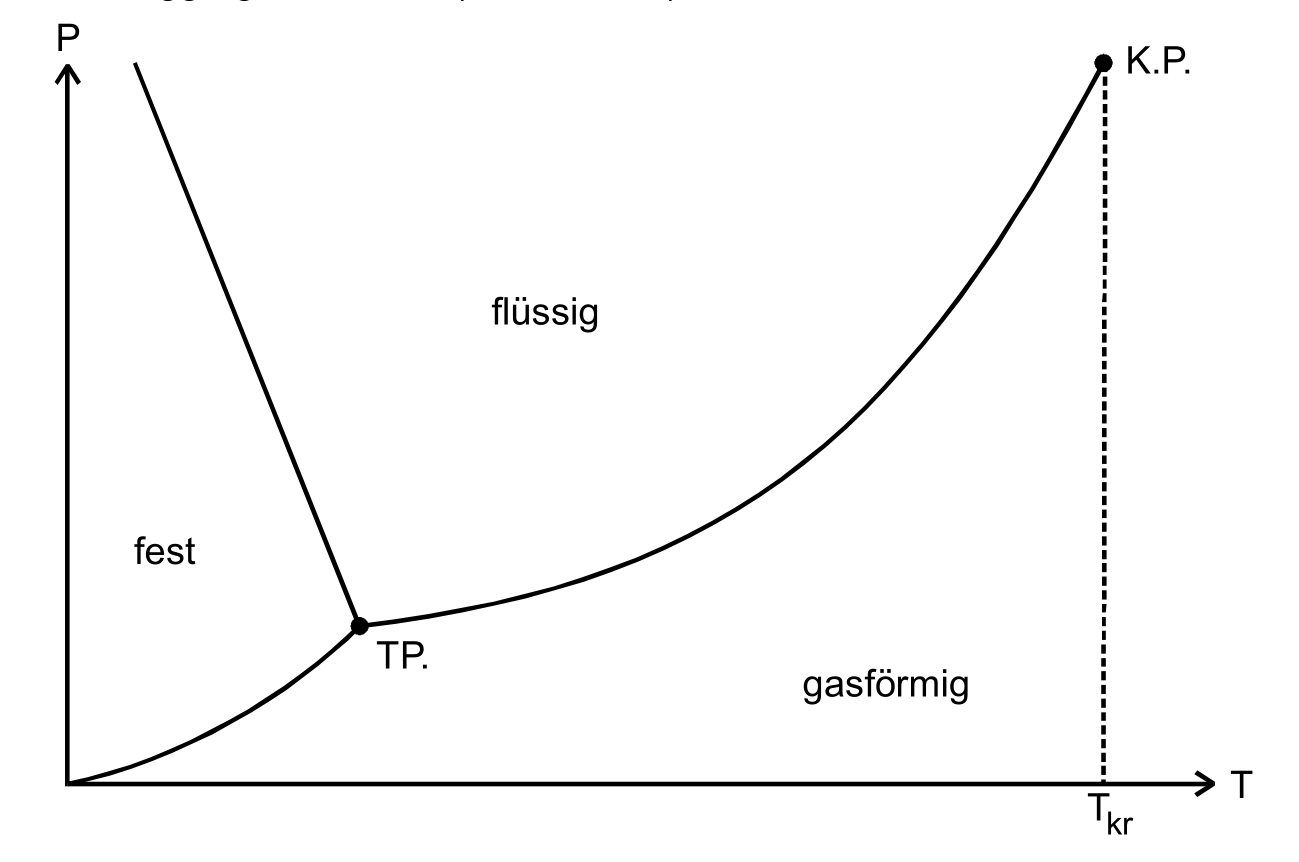
\includegraphics[width=0.55\textwidth]{images/Diagramm.PNG}
    \caption{Zustandsdiagramm des Wassers (qualitativ) \protect \cite{V203}.}
    \label{img:Zustand}
\end{figure}
\noindent Die beiden wichtigen Punkte in dem Diagramm sind der Tripelpunkt (TP.), indem die 
3 Aggregatzustände koexistieren und der kritische Punkt (K.P.) in dem der flüssige und gasförmige Zustand in einem 
thermodynamischem Gleichgewicht stehen.\\
In diesem Experiment wird jedoch nur der Übergang: flüssig $\Leftrightarrow$ gasförmig untersucht. 
Dieser Übergang wird von der Dampfdruckkurve beschrieben bzw. von der Siedepunktskurve zwischen dem Triplepunkt und dem kritischem Punkt.
Diese Kurve wird charakterisiert durch die temperaturabhängige Verdampfungswärme $L$. \\
Innerhalb jedes Stoffes werden die Geschwindigkeiten der einzelnen Teilchen
durch die Maxwellsche Geschwindigkeitsverteilung vorgegeben. Sobald die Geschwindigkeit eines Teilchen einen gewissen Grenzwert 
überschreitet, kann es aus der flüssig in die gasförmige Phase übergehen. Bei diesem Übergang müssen molekulare Bindungskräfte überwunden
werden. Dies ist die Verdampfungswärme $L$. Diese Energie wird beim Umkehrprozess, der Kondensation, wieder frei.\\
Zwischen der Kondensation und der Verdampfung entwickelt sich nach einiger Zeit ein Gleichgewicht.
Wenn genau so viele Moleküle aus der Flüssigkeit verdampfen wie aus dem Gas kondensieren, entsteht ein konstanter Druck.
Dies ist der Sättigungsdruck. $L$ ist eine temperaturabhängige Größe.
Allerdings gibt es einen Temperaturbereich in dem die Verdampfungswärme näherungsweise konstant ist.
Diesen Bereich nutzen wir in diesem Experiment um $L$ zu bestimmen.\\
Somit beschreibt die molare Verdampfungswärme $L$ eine stoffspezifische Größe, die angibt, wie viel Energie nötig ist,
um ein Mol einer Flüssigkeit isotherm und isobar zu verdampfen.\\
Der Sättigungsdruck lässt sich nicht durch die allgemeine Gasgleichung:
\begin{equation}
    pV=\text{R}T
    \label{eqn:Gasgl}
\end{equation}
mit dem Druck $p$, dem Volumen $V$, der Temperatur $T$ und der allgemeine Gaskonstante R=$\SI{8.314}{\joule\per\mole\kelvin}$ 
beschreiben, da der Sättigungsdruck nicht von dem Volumen des Gases, lediglich von den Temperaturen der Flüssigkeit 
und des Gases abhängen.
\\

\subsection{Kreisprozess}

\begin{figure}[H]
    \centering
    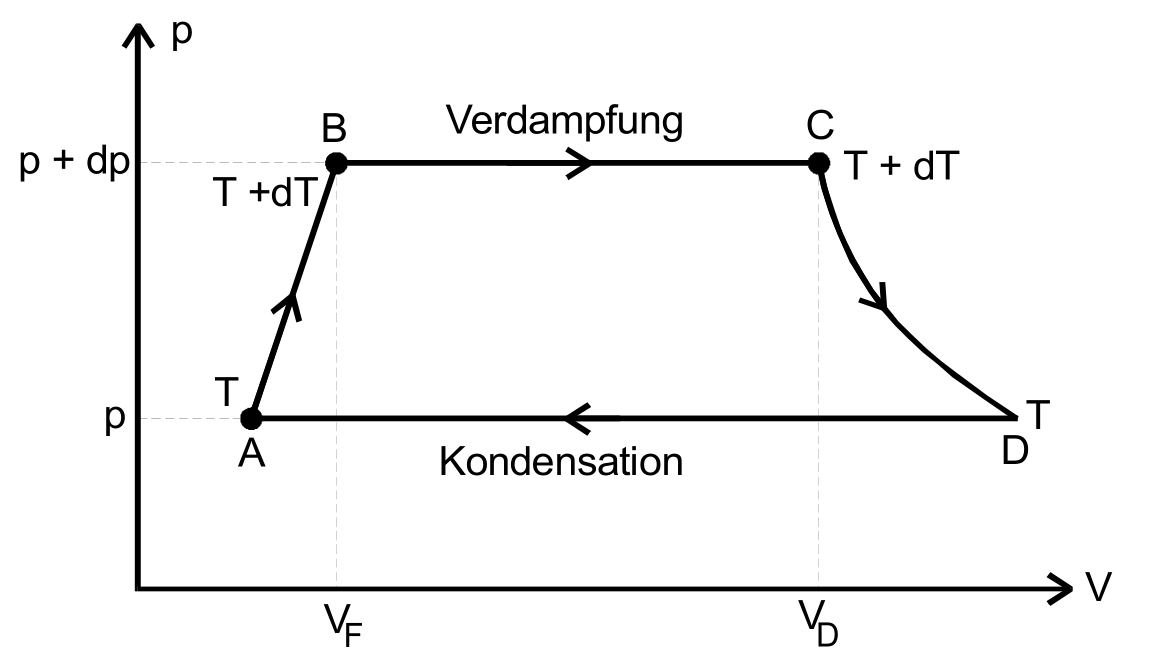
\includegraphics[width=0.55\textwidth]{images/Kreislauf.PNG}
    \caption{Darstellung eines Kreisprozesses im pV-Diagramm \protect \cite{V203}.}
    \label{img:Kreislauf}
\end{figure}

\noindent Um nun eine Dampdruckkurve zu erhalten, wird ein reversibler Kreisprozess analysiert. Hier findet in einem fortlaufendem 
Kreislauf eine isotherme und isobare Vedampfung gefolgt von einer isothermen und isobaren Kondensation statt.
Beim Ausgangspunkt A wird die Wärmemenge $\text{dQ}_\text{AB} $ hinzugeführt, so dass der Druck und die Temperatur um $\symup{d}p$ und $\symup{d}T$ ansteigen.
Diese Wärmemenge berechnet sich mittels der spezifischen Wärmekapazität der Flüssigkeit.

\begin{equation}
    \text{dQ}_\text{AB}= \text{C}_F \cdot dT \nonumber\\
\end{equation}
$\rightarrow$ Zustand B\\

\noindent Die Flüssigkeit aus Zustand B verdampft isobar und isotherm unter Aufnahme der Verdampfungswärme d$L$\\

\begin{equation}
L\text{(T + dT)} = L\text{(}T\text{) + d}L\nonumber\\
\end{equation}

\noindent Für diesen Prozess muss die Flüssigkeit eine gewisse Arbeit $\text{A}_\text{BC}$ verichten. Diese Arbeit bestimmt sich mit:\\

\begin{equation}
   - \text{A}_\text{BC} = \text{(}p + \text{d}p\text{)(}V_\text{D} - V_\text{F}\text{)} \nonumber
\end{equation}

$\rightarrow$ Zustand C\\
Der Dampf wird jetzt wieder auf die Temperatur T abgekühlt.
Bei diesem Schritt wird wieder eine gewisse Wärmemenge $\text{dQ}_\text{CD}$ frei:

\begin{align}
 -\text{dQ}_\text{CD} &=\text{C}_\text{D}\cdot \text{d}T & \text{C}_\text{D}&=\text{Molarwärme des Dampfes}  \nonumber 
\end{align}

$\rightarrow$ Zustand D\\
Im letzten Schritt kondensiert der Dampf unter Zufuhr einer gewissen mechanischen Arbeit $\text{A}_\text{Da}$.
Hierbei wird wiederum die Verdampfungswärme L(T) frei.

\begin{equation}
    -\text{A}_\text{DA}= p\cdot\text{(}V_\text{D} - V_\text{F}\text{)}  \nonumber
\end{equation}

$\rightarrow$ Zustand A\\

            %weiter Herleitung der Formel

\noindent Nach dem ersten Hauptsatz der Thermodynamik darf nun die Summe der insgesamt hinzugefügt Wärme mit der insgesamt 
verrichteten Arbeit gleichstellen. Dies ergibt dann:    

\begin{equation}
    (C_\text{F}-C_\text{D}\text{)d}T + \text{d}L = \text{(}V_\text{D}-V_\text{F}\text{)d}P\\
    \label{eqn:wearme=Arbeit}
\end{equation}

\noindent Weiterhin ist nach dem zweiten Hauptsatz der Thermodynamik die Summer der reduzierten Wärmemenge gleich 0.

\begin{equation}
    \sum_{i}\frac{Q_\text{i}}{T_\text{i}}=0\nonumber\\
\end{equation}

\noindent Außerdem dürfen wir die Differentialausdrücke 2. Ordnung vernachlässigen und erhalten dadurch:

\begin{equation} 
    \text{(C}_\text{F} - \text{C}_\text{D}\text{)d}T + \text{d}L -\frac{L\text{d}T}{T}= 0
    \label{eqn:Wearme=0}
\end{equation}

\subsection{Clausius-Clapeyronische Gleichung}

\noindent Das Gleichstellen der Formel \eqref{eqn:wearme=Arbeit} mit der Formel \eqref{eqn:Wearme=0} ergibt dann:

\begin{equation}
    (V_\text{D}-V_\text{F})\text{d}p =\frac{L}{T}\text{d}T\\
    \label{eqn:Clausius}
\end{equation}

\noindent Die erhaltene Formel \eqref{eqn:Clausius} wird in der Literataur als Clausius-Clapeyronische Gleichung bezeichnet. Mit ihrer Hilfe 
lässt sich die Dampfdruckkurve eines Stoffes berechnen. Da sich die Integration sehr schwierg gestalten kann, müssen zum Lösen
zunächst einige Näherungen gemacht werden. Diese gelten, in besonderen Temperaturbereichen.\\

        %Loesung der Clausius Gleichung
\noindent Für den Temperaturbereich weit unter der kritischen Temperatur $T_\text{kr}$ \\ (siehe Abbildung \ref{img:Zustand}) dürfen einige 
Näherungen gemacht werden.
\begin{enumerate}
    \item $V_F$ ist im Verhältnis zu $V_D$ vernachlässigbar.
    \item $V_D$ lässt sich durch die ideale Gasgleichung beschreiben \eqref{eqn:Gasgl}\\
            \begin{equation}
                \Rightarrow \text{V}_\text{D} \text{(p, }T\text{)} = \text{R} \cdot \frac{T}{p} \nonumber
            \end{equation}
    \item Die Verdampfungswärme $L$ ist druck- und temperaturunabhängig.
\end{enumerate}

\noindent Unter diesen Näherungen können die Clausius-Clapeyronsche Gleichung \eqref{eqn:Clausius} deutlich Vereinfachen werden:

\begin{equation}
    \frac{R}{\text{p}}\text{d}p = \frac{L}{T^2}\text{d}T \nonumber
\end{equation}
\begin{align}
p &= \text{exp}(C)\cdot \text{exp}\left(-\frac{L}{RT}\right) \nonumber\\
\text{ln}(p)&= -\frac{L}{RT} + C \nonumber
\end{align}

\noindent mit $C$ = ln($\text{p}_0$)
